\documentclass{article}
\usepackage{listings}
\usepackage{hyperref}
\usepackage{xcolor}
\usepackage{tikz}
\usepackage{float}
\usetikzlibrary{positioning, arrows.meta, shapes.geometric}

\hypersetup{
    colorlinks=true,
    linkcolor=blue,
    filecolor=magenta,      
    urlcolor=cyan,
    pdftitle={Overleaf Example},
    pdfpagemode=FullScreen,
    }

\urlstyle{same}

\lstset{
  basicstyle=\ttfamily,
  columns=fullflexible,
  breaklines=true,
  postbreak=\mbox{\textcolor{red}{$\hookrightarrow$}\space},
}

% Define colors
\definecolor{codegray}{gray}{0.9}

% Code listing style
\lstdefinestyle{mystyle}{
    backgroundcolor=\color{codegray},   
    commentstyle=\color{green},
    keywordstyle=\color{magenta},
    numberstyle=\tiny\color{codegray},
    stringstyle=\color{purple},
    basicstyle=\ttfamily\footnotesize,
    breakatwhitespace=false,         
    breaklines=true,                 
    captionpos=b,                    
    keepspaces=true,                 
    numbers=left,                    
    numbersep=5pt,                  
    showspaces=false,                
    showstringspaces=false,
    showtabs=false,                  
    tabsize=2
}

\lstdefinelanguage{yaml}{
  keywords={true,false,null,y,n},
  keywordstyle=\color{darkgray}\bfseries,
  basicstyle=\ttfamily,
  sensitive=false,
  comment=[l]{\#},
  commentstyle=\color{purple}\ttfamily,
  stringstyle=\color{red}\ttfamily,
  morestring=[b]',
  morestring=[b]"
}

\lstset{style=mystyle}

\begin{document}

\title{Docker Essentials: A Beginner's Guide to Modern Application Deployment}
\author{Shohruh MIRYUSUPOPV}
\date{\today}
\maketitle

\begin{abstract}
This tutorial offers a comprehensive introduction to Docker, a platform that has revolutionized software deployment by encapsulating applications into lightweight, portable containers. It demystifies the Docker ecosystem, explaining its core components—the Docker Client, Docker Daemon, and Docker Registry—and their interplay. Participants will learn how to set up Docker, create and manage containers, and understand the stark efficiencies Docker offers over traditional virtual machines. Aimed at beginners, this guide ensures that even those with no prior experience with Docker will gain the necessary skills to utilize container technology effectively, marking their first step into the world of modern, container-based application deployment.
\end{abstract}

\tableofcontents

\newpage
\section{Introduction}
\subsection{Understanding Docker: A Tour to History}

To grasp the fundamental concept of Docker, let's take a brief journey back in time. Imagine the era when goods were transported across the globe in barrels, crates, and various other containers. Each of these containers had its own unique size and shape. This diversity presented a significant challenge: unloading ships was a cumbersome and time-consuming task, which, in turn, increased the cost of shipping.

This scenario changed dramatically with the introduction of standardized shipping containers. These containers, uniform in size and shape, could be easily loaded, unloaded, and stacked on ships, trains, and trucks. This standardization not only streamlined the entire shipping process but also significantly reduced costs and improved efficiency.

Docker does something very similar in the world of software development and deployment. Just as standardized containers revolutionized the shipping industry by making it easier to transport goods globally, Docker containers revolutionize software development by making it easier to create, deploy, and run applications.

With Docker, applications are packaged along with their dependencies into containers, which are standardized units for software development. These containers ensure that applications run smoothly and consistently across any environment, from a developer's personal laptop to a high-capacity cloud server. This eliminates the common issue of encountering bugs or inconsistencies when moving software from one computing environment to another, a problem often summarized as "it works on my machine."

\subsection{Definitions and outline of tutorial}
This tutorial provides a brief introduction to Docker containerization with a focus on Windows containers. Docker is a platform that allows you to package your application and its dependencies into a container, which can then be run on any system that supports Docker. This ensures that your application works uniformly and consistently across any environment. First we give definitions used in the context of Docker and containerization \cite{docker}.

\begin{description}
    \item \textbf{Docker Image}: A Docker image is a lightweight, standalone, executable package that includes everything needed to run a piece of software, including the code, runtime, libraries, environment variables, and config files. The image file is created from \texttt{.Dockerfile}.
    \item \texttt{.Dockerfile}: The starting point in the Docker containerization process. It contains a set of instructions to build a Docker image, specifying the base image, software installations, configurations, and the application to run.
    \item \textbf{Docker Container (Ephemeral)}: A container is a runtime instance of a Docker image. It runs completely isolated from the host system by default, only accessing files and ports if configured to do so.  It is described as "ephemeral" to underline that it is temporary and designed to perform specific tasks or run specific applications and then be destroyed. This ensures a clean, predictable environment for each execution.
    \item \textbf{Volume Mounting}: This refers to the process of attaching a volume (a designated directory on the host or in the cloud) to a container, allowing for data persistence and sharing between containers.
    \item \textbf{Container Logs}: Logs provide insights into the operations and events happening within a container. They are crucial for debugging and monitoring the behavior of applications running inside containers.
    \item \textbf{Docker Commands}: Throughout the tutorial, we will use various Docker commands to manage images, containers, and volumes. These commands allow you to build, run, stop, and remove containers and images, as well as inspect logs and manage volumes.
    \item \textbf{Docker volume}: A volume is a persistent data storage mechanism that allows data to be kept in a designated area outside the container's filesystem. This means that the data in the volume can survive container restarts and can be shared between multiple containers. Volumes are managed by Docker and are stored on the host filesystem, but they are managed in a way that is more flexible and secure than simply mounting a host directory into a container. Volumes can be used for various purposes, such as storing database files, unique configurations, or any data that should persist or be accessible across container instances.
\item[Docker Daemon] It is often referred to as \texttt{dockerd}, is a background service that manages the entire Docker lifecycle of containers and images. It listens for Docker API requests and manages Docker objects such as images, containers, networks, and volumes.
\begin{itemize}
\item When building an image, the Daemon assembles the image based on the instructions in the Dockerfile.
\item For pulling an image, the Daemon fetches the specified image from the Docker registry.
\item To run a container, the Daemon instantiates an instance of an image, providing an isolated environment for its execution.
\end{itemize}
\item[Docker Host] it is the machine on which the Docker Daemon runs. It's responsible for running containers and managing Docker services.
\item[Docker Client] The Docker Client is the user interface to Docker. It provides the means for users to interact with Docker via the command line using commands such as docker build, docker pull, and docker run. When a command is issued from the client:
\begin{itemize}
\item \texttt{docker build} sends a request to the Docker Daemon to build an image from a Dockerfile.
\item \texttt{docker pull} asks the Docker Daemon to pull an image from a registry.
\item \texttt{docker run} requests the Docker Daemon to run a container from an image.
\end{itemize}
\item[Registry] The Registry is a storage and content delivery system, holding Docker images. Docker Hub is a public registry that anyone can use, and Docker is configured to look for images on Docker Hub by default. Private registries can also be used.
\end{description}

We will go through the process of building a Docker image, running a container with volume mounting, and inspecting logs and volumes. This tutorial is designed for beginners and aims to provide a practical understanding of Docker containerization on Windows.

\section{Docker Pipeline and Architecture}

\subsection{Main Pipeline}
This diagram illustrates the process of creating and running a Docker container, emphasizing the ephemeral nature of containers and the persistent storage provided by Docker volumes.

\begin{figure}
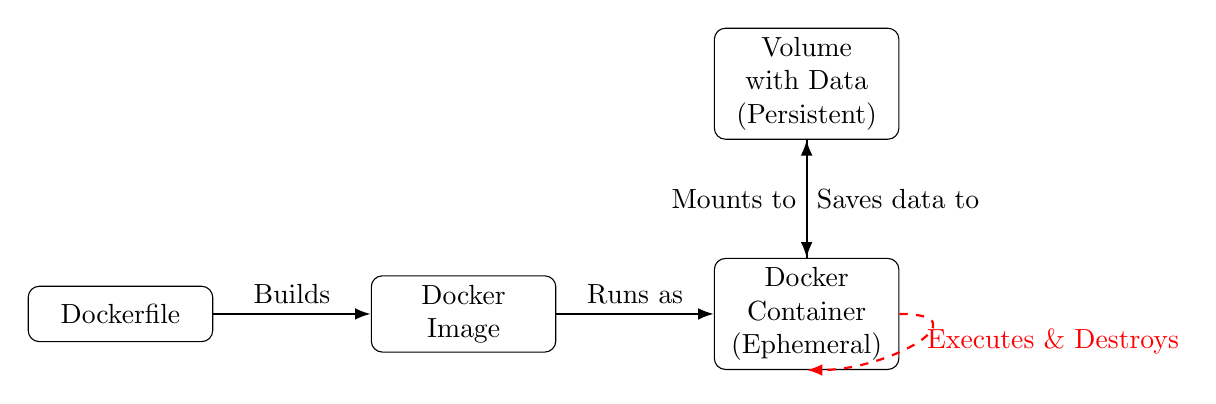
\begin{tikzpicture}[
    node distance=1.5cm and 2cm,
    auto,
    block/.style={
        rectangle,
        rounded corners,
        draw=black,
        text width=6em,
        align=center,
        minimum height=2em
    },
    arrow/.style={
        ->,
        thick,
        -{Latex[length=2mm]}
    },
    save/.style={
        -{Latex[length=2mm]}, dashed, thick
    },
    lifecycle/.style={
        -{Latex[length=2mm]}, dashed, thick, red
    }
]

% Nodes
\node[block] (dockerfile) {Dockerfile};
\node[block, right=of dockerfile] (image) {Docker Image};
\node[block, right=of image] (container) {Docker Container (Ephemeral)};
\node[block, above=of container] (volume) {Volume with Data (Persistent)};

% Arrows
\draw[arrow] (dockerfile) -- (image) node[midway, above] {Builds};
\draw[arrow] (image) -- (container) node[midway, above] {Runs as};
\draw[arrow] (volume) -- (container) node[midway, left] {Mounts to};
\draw[save] (container) -- (volume) node[midway, right] {Saves data to};

% Lifecycle notation
\draw[lifecycle] (container.east) to[out=0,in=0,looseness=2] node[right] {Executes \& Destroys} (container.south);
\end{tikzpicture}
\caption{Docker's main pipeline.}
\end{figure}

\begin{description}
\item[Builds]: The Dockerfile is used to build the Docker Image, encapsulating the application and its environment.
Runs as: The Docker Image then serves as the basis for creating an ephemeral Docker Container, which is executed to run the application.
\item[Mounts to]: A Volume with Data is mounted to the Docker Container, providing a persistent storage solution that allows the container to read from and write data to a persistent storage area.
\item[Saves data to]: Data generated or modified by the application running in the container is saved back to the Volume. This ensures that important data is not lost when the container is destroyed.
\item[Executes \& Destroys]: Highlighting the lifecycle of the container, this loop indicates that after the container has executed its task, it can be destroyed. The destruction of the container does not affect the persistence of data stored in the volume, which can be reused or accessed by future containers.
\end{description}

\subsection{Comparison to Virtual Machines}

\begin{figure}[H]
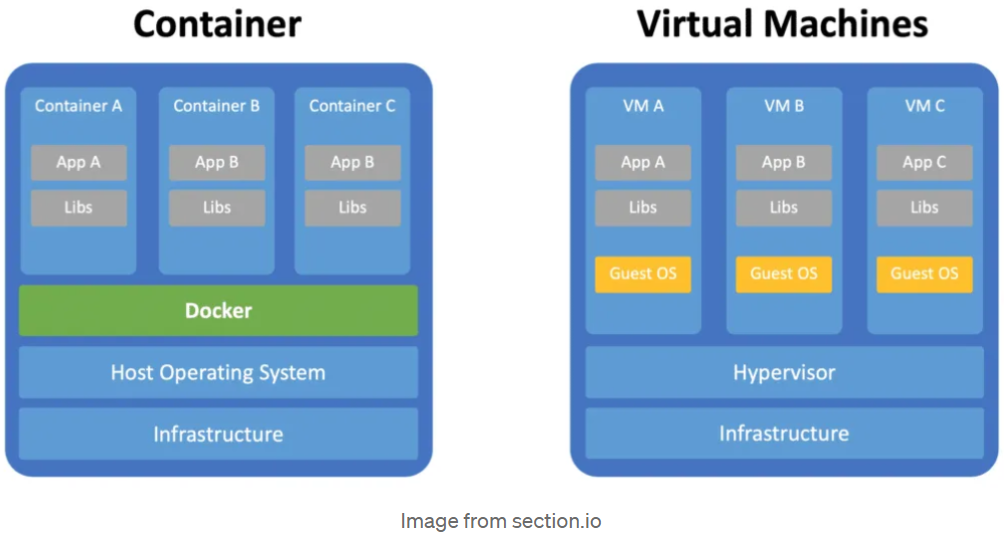
\includegraphics[scale=.45]{figures/docker_vm.png}
\caption{Dockers architecture}
\label{fig:docker_vm}
\end{figure}

On the left of Figure \ref{fig:docker_vm}, the "Container" section illustrates how containers operate. Multiple containers, labeled as Container A, B, and C, are shown each containing an application (App A, B, and B, respectively) and its libraries (Libs). These containers all share the same host operating system, which is indicated directly below the containers, and in turn, the host OS runs directly on the infrastructure. On the right, the "Virtual Machines" section shows a setup with three separate VMs (VM A, B, and C). Each VM runs its own application and libraries, similar to the containers. However, each VM also includes a guest operating system. These guest OS instances are individual for each VM, which adds additional overhead.  Containers share the same OS kernel and isolate the applications at a higher level, which can result in better resource utilization and faster startup times compared to VMs. 

\subsection{Docker's Architecture}

Figure \ref{fig:docker_arch} provides a high-level overview of the Docker architecture, illustrating the process from image creation or acquisition to the running of containers, all coordinated by the Docker Daemon in response to commands issued by the Docker Client. 

The client is where Docker users execute commands. When a user issues a docker build command, the client sends this instruction to the Docker Daemon, which resides on the Docker host. The Docker Daemon processes this command and builds an image, which it can then push to a registry—a service that hosts and distributes Docker images. Similarly, when the client issues docker pull, it instructs the Docker Daemon to fetch an image from the registry and store it locally on the Docker host. Finally, the docker run command tells the Docker Daemon to create a new container from a specified image. The container is a runtime instance of an image and executes on the Docker host.

\begin{figure}[H]
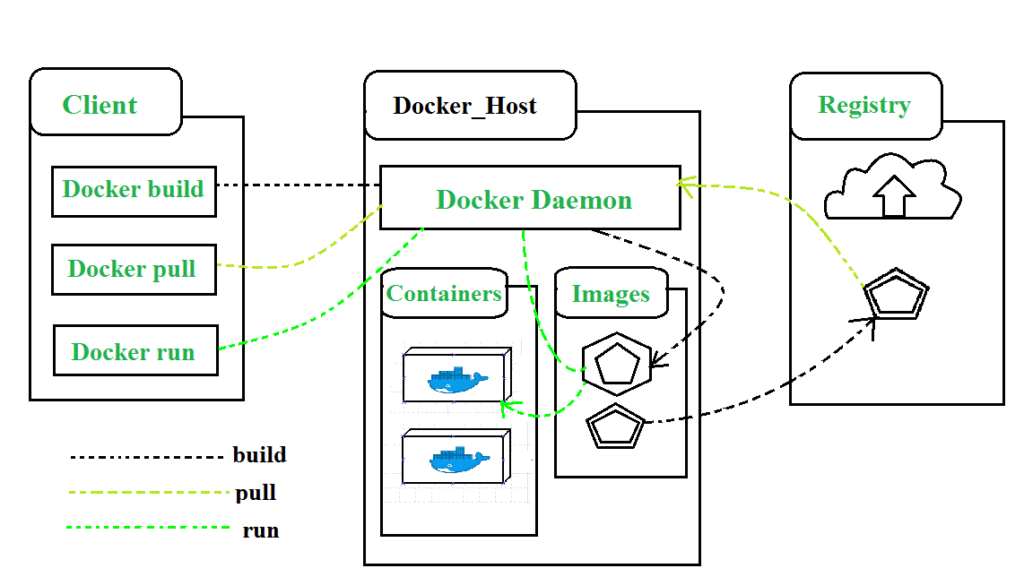
\includegraphics[scale=.37]{figures/docker_architecture.png}
\caption{Dockers architecture \cite{geeksDocker}}
\label{fig:docker_arch}
\end{figure}

\section{Building the Docker Image}
All the instructions are passed through Docker Client. Once Docker is installed, they can open PowerShell (on Windows), Terminal (on macOS), or any other command-line interface to interact with Docker using the Docker Client. It is through this interface that users will send commands to the Docker Daemon to manage the lifecycle of containers and images.

To build a Docker image, especially one that requires Python libraries, we need to include a requirements.txt file in our build context. This file lists all the Python dependencies that need to be pre-installed in the image. When building the image, we can specify a GitHub token as a build argument to allow access to private repositories if necessary. The image can then be tagged as \texttt{my-app}. Including the \texttt{requirements.txt} ensures that the resulting Docker image is pre-equipped with the necessary Python libraries for the application to run properly.

\begin{lstlisting}
# Build a Docker image from a Dockerfile
# --build-arg: Passes the build-time variable GITHUB_TOKEN 
# with a value of 'sometoken'
# -t: Tags the resulting image as 'my-app'
# .: Indicates that the build context is the current directory,
# containing the Dockerfile
docker login
docker build --build-arg GITHUB_TOKEN=sometoken -t my-app .
\end{lstlisting}

\begin{itemize}
\item Hardcoding the GitHub token, or any sensitive information, directly in your build commands or Dockerfiles is not recommended due to security risks. Anyone who has access to your Dockerfile or command history could potentially extract this sensitive token. 
\item The docker build command should be executed in the directory where the \texttt{.Dockerfile} is located. This directory is referred to as the "build context." By specifying \texttt{.} at the end of the command, you are telling Docker that the build context is the current directory. This means all the files and directories in the current directory are available to the Docker daemon to build the image. An example of \texttt{.Dockerfile} can be found in Appendix \ref{dockerfile}.
\end{itemize}


\section{Running and Managing the Container}

\subsection{Running the Container}
With our image built, we can now run a container from it. We will create a volume named \texttt{test\_vol} and mount it to the container's \texttt{C:/data} directory. We will also allocate 45 GB of memory to our container and start a PowerShell session.

\begin{lstlisting}
# Create a new Docker volume named test_vol
docker volume create test_vol

# Run a container using the test-app image
docker run \
  -v test_vol:C:/data \ # Mount the volume test_vol 
  # to C:/data in the container
  --name test_container \ # Name the container test_container
  --memory 45g \ # Allocate 45 GB of memory to the container
  -it \ # Interactive mode with a tty
  test-app \ # Image name to use
  powershell # Start a PowerShell session inside the container
\end{lstlisting}

\begin{itemize}
\item \texttt{-v test\_vol:C:\textbackslash{}data}: Mounts the previously created volume \texttt{test\_vol} to the \texttt{C:\textbackslash{}data} directory inside the container. This allows for data persistence and sharing between the host and the container.
\item \texttt{--name test\_container}: Assigns the name \texttt{test\_containe}r to the new container. This makes it easier to manage the container using Docker commands.
\item \texttt{--memory 45g}: Specifies the amount of memory that the container is allowed to use. In this case, the container is allocated 45 GB of memory.
\item \texttt{-it}: Runs the container in interactive mode with a tty (terminal), enabling interaction with the container.
\item \texttt{test-app}: Specifies the name of the image to create the container from. In this context, test-app is the name of the Docker image that was previously built.
\item \texttt{powershell}: Specifies that a PowerShell session should be started within the container. This allows for interactive management of the container using PowerShell commands.
\end{itemize}


\subsection{Managing Containers and Images}
To manage our Docker containers and images, we can use various Docker commands:

\begin{lstlisting}
# List all running containers
docker ps

# Stop a running container
docker stop my-container

# View logs of a container
docker logs my-container
docker logs -f my-container

# Remove a stopped container
docker rm my-container

# List all Docker images
docker images

# Remove an image
docker rmi my-app1
docker rmi -f c6cc01e60919

# Start a PowerShell session in a new container
docker run -it --entrypoint powershell my-app

# Execute PowerShell in a running container
docker exec -it my-container powershell
\end{lstlisting}

\section{Working with Volumes}

\subsection{Managing volumes}

There are three main types of mounts shown that connect the container to storage resources \cite{dockerstorage}:

\begin{itemize}
\item Bind Mount: This connects a specific directory or file on the host machine's filesystem to a path within the Docker container, allowing the container to read from and write to the host's filesystem directly.

\item Volume: This is a Docker-managed portion of the filesystem that is abstracted from the host, providing a persistent and container-agnostic way to store data. Volumes are not tied to the specific container that creates them, so they can be easily shared among multiple containers.

\item tmpfs Mount: This storage option mounts a temporary file storage facility directly into the container's memory space. It is backed by the host machine's memory, but unlike bind mounts and volumes, a tmpfs mount is temporary and is deleted when the container stops.

Figure \ref{fig:docvol} showcases the different storage options available for a Docker container. 
\end{itemize}
\begin{figure}[h!]
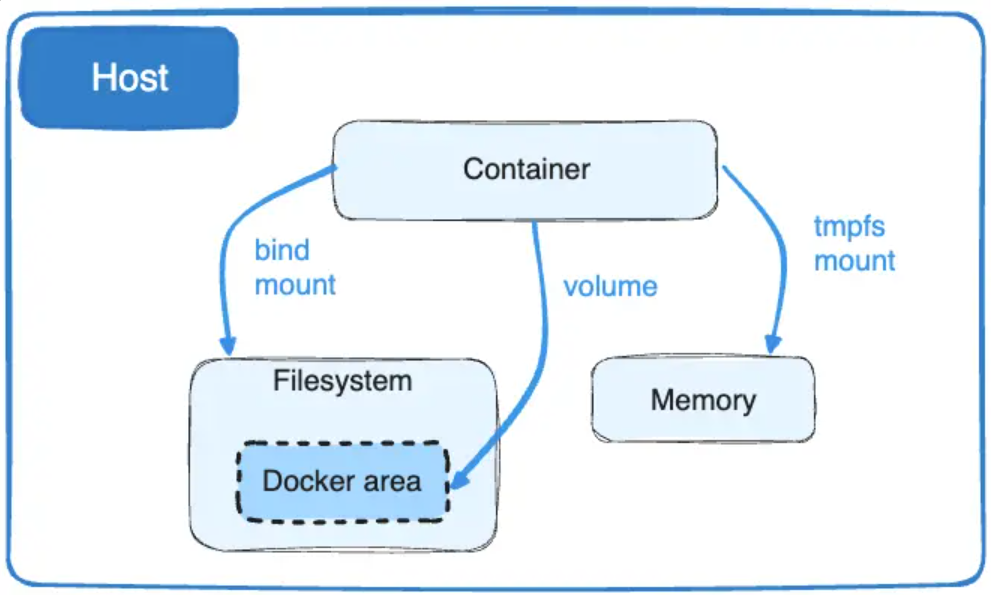
\includegraphics[scale=.5]{figures/docker_volume.png}
\caption{Docker Container Storage Options \cite{dockervol}}
\label{fig:docvol}
\end{figure}


To create a Docker volume, you use the docker volume create command followed by the name of the volume. This command creates a new volume that can be mounted into containers to persist data.

\begin{lstlisting}
docker volume create test_vol
\end{lstlisting}

To see a list of all volumes on your Docker host, use
\begin{lstlisting}
docker volume rm test_vol
\end{lstlisting}

We can inspect a volume to get detailed information about it
\begin{lstlisting}
docker volume inspect test_vol
\end{lstlisting}

To remove a Docker volume, which is useful for cleaning up unused or temporary data, you use the docker volume rm command followed by the name of the volume. It's important to ensure that no containers are currently using the volume you wish to remove.
\begin{lstlisting}
docker volume rm test_vol
\end{lstlisting}

\subsection{Create container with mounted volume}
To create and work with Docker volumes, we use the following commands:

\begin{lstlisting}
# Create a new container with a volume mounted
docker run \
  # Assign the name temp-container to the new container
  --name temp-container \
  # Mount the volume my_app_volume to C:\data in the container
  -v my_app_volume:C:\data \ 
  -it \ # Interactive mode with a tty
  # Image to use: Windows Server Core LTSC 2019
  mcr.microsoft.com/windows/servercore:ltsc2019 \
  cmd # Start the container with a command prompt session
\end{lstlisting}

\begin{itemize}
\item --name temp-container assigns the name temp-container to the new container for easier reference.
\texttt{-v my\_app\_volume:C:\textbackslash{}data} mounts the \texttt{my\_app\_volume} volume to the container's \texttt{C:\textbackslash{}data} directory, allowing for data persistence between container restarts or sharing data among multiple containers.
\item \texttt{-it} indicates that the container should be run in interactive mode with a terminal session (tty), allowing you to interact with the container's command prompt directly.
\item \texttt{mcr.microsoft.com/windows/servercore:ltsc2019} specifies the base image for the container. In this case, it's the Windows Server Core LTSC 2019 image from Microsoft's Container Registry.
\item \texttt{cmd} is the command to start a command prompt session inside the container, allowing you to execute further commands within the container's environment.
Following the docker run command, the docker volume inspect command is used to retrieve detailed information about the specified volume, \texttt{my\_app\_volume}. 
\end{itemize}

\subsection{Why Volumes and not Bind Mounts?}
Volumes have several advantages over bind mounts \cite{dockervol}:
\begin{itemize}
\item Portability: Volumes are simpler to backup and transfer between systems compared to bind mounts.

\item Manageability: Volumes can be managed with Docker CLI or API, providing a user-friendly approach to handling storage.

\item Compatibility: Volumes are compatible with both Linux and Windows containers, offering a versatile solution for container data.

\item Sharing: Volumes can be securely shared among multiple containers, which is less risky than sharing bind mounts.

\item Extensibility: Volume drivers allow for the expansion of functionality, including storage on remote systems, encryption, and more.

\item Initialization: New volumes can be pre-filled with data from a container, making setup processes more efficient.

\item Performance: On Docker Desktop for Mac and Windows, volumes perform significantly better than bind mounts.
\end{itemize}


\section{Summary}
This tutorial covered the basics of Docker containerization on Windows, including image creation, container management, and volume handling.

\appendix

\section{Dockerfile manifest} \label{dockerfile} \index{\texttt{.Dockerfile}}

This \texttt{.Dockerfile} is designed for creating a Windows-based Docker image that sets up a Python development environment with Git, and is tailored for deploying a Python application.


\begin{lstlisting}[language=yaml]
# Use a Windows base image
ARG GITHUB_TOKEN

FROM mcr.microsoft.com/windows/servercore:ltsc2022

# Set the working directory in the container
WORKDIR C:\\myapp

# Use PowerShell for subsequent commands
SHELL ["powershell", "-Command", "$ErrorActionPreference = 'Stop';"]

# Install Python and Git
# Note: Replace the URLs with the actual URLs for Python and Git installers
RUN Invoke-WebRequest -Uri 'https://www.python.org/ftp/python/3.9.0/python-3.9.0-amd64.exe' -OutFile 'python_installer.exe' -UseBasicParsing; \
    Start-Process python_installer.exe -ArgumentList '/quiet InstallAllUsers=1 PrependPath=1' -Wait; \
    Remove-Item python_installer.exe -Force; \
    Invoke-WebRequest -Uri 'https://github.com/git-for-windows/git/releases/download/v2.28.0.windows.1/Git-2.28.0-64-bit.exe' -OutFile 'git_installer.exe' -UseBasicParsing; \
    Start-Process git_installer.exe -ArgumentList '/VERYSILENT /NORESTART /NOCANCEL /SP-' -Wait; \
    Remove-Item git_installer.exe -Force
    # Invoke-WebRequest -Uri 'https://curl.se/ca/cacert.pem' -OutFile 'cacert.pem'; \
    # [System.Environment]::SetEnvironmentVariable('GIT_SSL_CAINFO', 'C:\codpy\cacert.pem', [System.EnvironmentVariableTarget]::Machine); \
    # Remove-Item cacert.pem -Force

# Add Python and Git to PATH (replace with the actual installation paths if different)
RUN $env:Path += ';C:\\Program Files\\Python39;C:\\Program Files\\Python39\\Scripts;C:\\Program Files\\Git\\cmd'; \
    [Environment]::SetEnvironmentVariable('Path', $env:Path, [EnvironmentVariableTarget]::Machine)

# Set the GitHub token as an environment variable
ENV GITHUB_TOKEN=$GITHUB_TOKEN

# Use the token to install the codpy package from the private repository
RUN $Env:GITHUB_TOKEN='YOURGITHUBTOKEN'; \
    git clone https://yourrepo:$Env:GITHUB_TOKEN@github.com/yourrepo/myapp.git; \
    cd myapp; \
    pip install .

# Reset the working directory to C:\app
WORKDIR C:\\app

# Copy the content of the local src directory to the working directory
COPY . C:\\app

# Install any dependencies from requirements.txt
RUN pip install --no-cache-dir -r requirements.txt

# If necessary,  copy the specific .pyd file to the site-packages directory
COPY ["yourapp.cp39-win_amd64.pyd", "C:/Program Files/Python39/Lib/site-packages/"]

# Command to run on container start
#CMD ["powershell", "-Command", "while ($true) { Start-Sleep -Seconds 3600 }"]

CMD ["python", "C:\\app\\main.py"]
\end{lstlisting}


\begin{description}
\item[Base Image]: The image starts from a Windows Server Core base image (\texttt{ltsc2022}). This provides the underlying Windows operating system environment.

\item[Working Directory]: It sets the working directory inside the container to \texttt{C:/\ myapp}, which is where subsequent commands will operate.

\item[Shell Setting]: The shell is set to PowerShell with error preferences, ensuring that subsequent commands are run using PowerShell and that any errors stop the process.

\item[Python and Git Installation]: It installs Python and Git by downloading their installers from specified URLs and running them silently. After installation, the installers are removed to keep the image size down.

\item[Path Environment Variable]: The \texttt{Dockerfile} appends the Python and Git executable paths to the system PATH environment variable, allowing these programs to be run from any location within the container.

\item[GitHub Token]: Sets an environment variable \texttt{GITHUB\_TOKEN} using the build argument \texttt{ARG GITHUB\_TOKEN}, which is intended to be used for secure access to private repositories.

\item[Clone and Install Python Application]: It uses the provided GitHub token to clone a Python application from a private GitHub repository. Then it changes to the application directory and installs it using pip. This process assumes that the application has a setup.py file for installation.

\item[Reset Working Directory]: The working directory is reset to \texttt{C:/\ app}.

\item[Copy Application Files]: Copies the application files from the local source directory to the container's working directory.

\item[Install Dependencies]: Installs any dependencies specified in requirements.txt using pip.

\item[Copy \texttt{.pyd} File]: If necessary, copies a specific \texttt{.pyd} file (a Python extension module) to the Python site-packages directory, which is where Python looks for installed packages.

\item[Set Startup Command]: Finally, it sets the default command to run the Python application (main.py) located at \texttt{C:/\ app/\ main.py} when the container starts.
\end{description}

\section{Example of \texttt{requirements.txt} File}

\begin{lstlisting}[language=yaml]
scipy
torch
torchvision>=2.0.1
numpy
\end{lstlisting}

\begin{thebibliography}{1}
\bibitem{dockervol} \href{https://docs.docker.com/storage/volumes/}{Docker Docs: Volumes, Docker documentation}
\bibitem{docker} Docker's glossary. \url{https://docs.docker.com/glossary/}
\bibitem{dockerbuild} \href{https://docs.docker.com/engine/reference/commandline/image_build/}{Docker docs: docker build (docker image build)}
\bibitem{docker_use} \href{https://www.docker.com/resources/what-container/}{Use containers to Build, Share and Run your applications}
\bibitem{geeksDocker} \href{https://www.geeksforgeeks.org/features-of-docker/}{geeksforgeeks: Features of Docker}
\bibitem{dockerstorage} \href{https://docs.docker.com/storage/}{Docker docs: Manage data in Docker}
\end{thebibliography}

\end{document}
